\documentclass[a4paper,parskip]{scrartcl}

\usepackage{lmodern}
\renewcommand*\familydefault{\sfdefault}
\usepackage[T1]{fontenc}

\usepackage[ngerman]{babel} %german english spell checking
\usepackage[utf8]{inputenc} %allows ä,ö,ü and others
\usepackage{multicol} %allows multiple columns
\usepackage{enumitem} %allows to change enumerate style
\usepackage[colorlinks=true,pdfborder={0 0 0},urlcolor=cyan,linkcolor=black]{hyperref} %allows links
\usepackage{verbatim} %allows code
\usepackage{graphicx} %allows images
\usepackage{amssymb} %allows symbols for number sets
\usepackage[table]{xcolor}
\setlist{nosep} %smaller lists, less space between lines

\title{Anforderungs- Dokumentation}
\author{Lorenz Rasch \& Dominik Meister}

\begin{document}
\maketitle
\tableofcontents
\pagebreak

\section{Ziel des Dokumentes}
Dieses Dokument umschreibt die Anforderungen und Ziele für das Projekt 1, Mindmap. Es umschreibt
die Vision und die funktionellen und nicht funktionellen Anforderungen des Projektes.

\section{Vision}
Jeder kennt diese Situation, man sitzt in einem Meeting und möchte kurz ein Brainstorming machen. Oder man
möchte für die nächste Arbeit zu einem Thema eine Übersicht zu den Informationen erstellen.
Eine der einfachsten Methoden so eine Übersicht darzustellen ist das Mindmap. Das Mindmap auch Gedankenlandkarte genannt ist eine Technik welche von Tony Buzan geprägt und entwickelt wurde.
Das Mindmap basiert auf dem Prinzip der Assoziation. Dies kommt nicht von ungefähr, unser Gehirn arbeitet ebenfalls mit Assoziationen, es versucht ständig neue Informationen mit gewissen Kategorien und anderen Informationen zu verknüpfen. Das Mindmap basiert auf derselben Technik, deshalb fällt es uns auch sehr einfach ein Mindmap zu erstellen.
Dieses zu erstellen ist jedoch mit den meisten Programmen eher mühsam, deshalb greift man auf den Stift und Papier zurück. Um hier Abhilfe zu schaffen kommt unser Projekt ins Spiel.
\newpage
\section{Ziel des Projektes}
Ziel des Projektes ist es ein Mindmap Programm zu schreiben welches eine alternative zum Stift und Papier,
bietet. Die Mindmap Softwares sind gegenüber der Papiervariante umständlicher, es bietet aber dafür andere
Vorteile. Durch das Mindmap Programm gehen die Zeichnungen nicht so einfach verloren und können einfach 
in Dokumente eingebettet werden und versendet werden. Deshalb sind die Hauptziele des Projektes, 
die Einfachheit des Programmes.  

\subsection{SMART Ziele}
\begin{itemize}
\item Die Mindmaps müssen einfach abspeicherbar sein, damit es wieder geladen oder gesendet werden kann. 
\item Das System soll einfach zu bedienen sein, ein neuer Benutzer soll das Programm ohne weitere Hilfe
direkt bedienen können.
\item Durch die Einführung des neuen Programmes soll das verlieren von Mindmaps und somit Zeitverluste
minimiert werden. 
\item Der Benutzer sollte das Programm ohne weitere Hilfe direkt auf seinem PC ausführen können, eine Installation ist nicht notwendig.
\item Die Stakeholder des Projektes werden alle 2 Wochen über den Stand des Projektes informiert. Allfällige Anpassungen werden dann entgegengenommen.
\item Bis zum Projektende steht dem Stakeholder eine Dokumentation über das Programm mit Ablaufdiagrammen und UML Diagrammen zur Verfügung.

\end{itemize}
\newpage


\section{System Kontext}
Der Systemkontext ist eine Beschreibung des Systems, seiner Teile und äusserlichen Einwirkungen auf das System.
Der Benutzer kann mit unserer Software ein Mindmap erstellen. Dies geschieht über eine grafische Benutzeroberfläche. Mit Hilfe eines Algorithmus können die Themen und Verbindungen des Mindmap optimal verteilt werden. Die Benutzeroberfläche und der Algorithmus sind Teil der Software\\
Die Software greift auf das Dateisystem des Computers zu um ein Mindmap zu speichern oder zu laden.
Der Druckservice des Computers erlaubt das Drucken des Mindmaps. Diese beiden Teile liegen ausserhalb unserer Software.

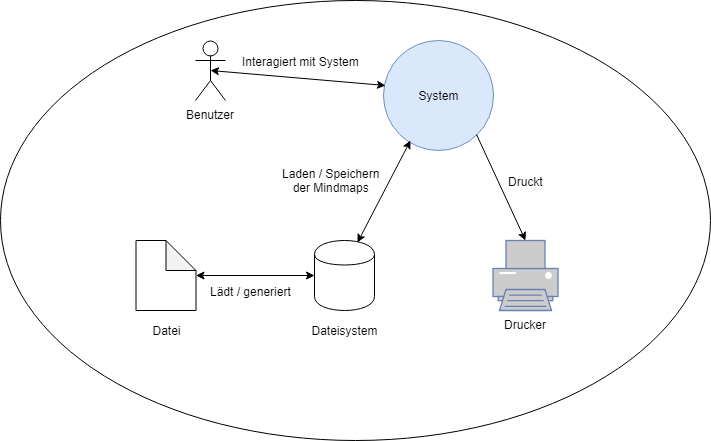
\includegraphics[width=1\linewidth]{images/Systemkontext.jpg}

\newpage

\section{Anforderungen}

\subsection{Nichtfunktionale Anforderungen}
Die Anforderungen werden mit den PKVR Werten bewertet. \\
P = Priorität  \\
K = Komplexität \\
V = Variablität \\
R = Risiko aus PKV \\ 
R = \(1/6P+1/3V+1/2K\) \\  
\\
Skala: 1 = niedrig, 2 = mittel, 3 = hoch \\


\begin{table}[h]

\begin{tabular}{|l|l|l|l|l|l|l|}

\hline
Nr  & Datum   & Beschreibung                 & P & K & V & R \\ \hline
NFA-1 & 14.3.19 & Benutzerfreundlich           & 3 & 1 & 3 & \cellcolor{yellow!20}2 \\\hline
NFA-2 & 14.3.19 & Schnell / Effizient          & 2 & 2 & 1 & \cellcolor{yellow!20}1.67 \\\hline
NFA-3 & 14.3.19 & Optisch ansprechendes Design & 1 & 2 & 3 & \cellcolor{red!20}2.17 \\\hline
NFA-4 & 14.3.19 & Output wie Input             & 3 & 1 & 1 & \cellcolor{green!20}1.33 \\\hline
NFA-5 & 14.3.19 & Einfache Installation        & 3 & 1 & 1 & \cellcolor{green!20}1.33 \\\hline
\end{tabular}
\end{table}
\begin{itemize}
\item[NFA-1]	Als Benutzer möchte ich, dass das Programm selbsterklärend und einfach zu bedienen ist. 
\item[NFA-2]	Als Benutzer möchte ich ein Programm welches schnell startet und sich nicht langsam anfühlt. 
\item[NFA-3]	Als Benutzer möchte ich ein optisch ansprechendes Design. Als Benutzer finde ich ein Programm besser wenn sein Design State of the Art ist. 
\item[NFA-4]	Als Benutzer möchte ich, dass das Mindmap auf dem Papier gleich aussieht wie es im Programm ausgesehen hat. 
\item[NFA-5]	Als Benutzer möchte ich nicht einen Experten konsultieren müssen um ein so triviales Programm zu installieren. 
\end{itemize}
\subsection{Funktionale Anforderungen}
\begin{table}[h]

\begin{tabular}{|l|l|l|l|l|l|l|}

\hline
Nr  & Datum   & Beschreibung                        & P & K & V & R \\ \hline
FA-1 & 14.3.19 & Neues Mindmap erstellen             & 3 & 1 & 1 & \cellcolor{green!20}1.33 \\\hline
FA-2 & 14.3.19 & Knoten hinzufügen                   & 3 & 1 & 1 & \cellcolor{green!20}1.33 \\\hline
FA-3 & 14.3.19 & Knoten miteinander verbinden        & 3 & 2 & 1 & \cellcolor{yellow!20}1.83 \\\hline
FA-4 & 14.3.19 & Mindmaps speichern/laden            & 2 & 2 & 2 & \cellcolor{yellow!20}2 \\\hline
FA-5 & 14.3.19 & Beschreibung eines Knoten anpassen  & 2 & 2 & 1 & \cellcolor{yellow!20}1.67 \\\hline
FA-6 & 14.3.19 & Farbe eines Knoten ändern           & 1 & 2 & 1 & \cellcolor{yellow!20}1.5 \\\hline
FA-7 & 14.3.19 & Verschiedene Verbindungstypen       & 1 & 1 & 1 & \cellcolor{green!20}1 \\\hline
FA-8 & 14.3.19 & Drucken eines Mindmaps              & 1 & 1 & 1 & \cellcolor{green!20}1 \\\hline
FA-9 & 14.3.19 & Exportieren eines Mindmaps          & 2 & 2 & 2 & \cellcolor{yellow!20}2 \\\hline
FA-10 & 14.3.19 & Optimale Verteilung der Knoten     & 1 & 3 & 1 & \cellcolor{yellow!20}2 \\\hline

\end{tabular}

\end{table}

\begin{enumerate}
\item[FA-1] Als Benutzer möchte ich mit dem Programm neue Mindmaps erstellen können.
\item[FA-2] Als Benutzer möchte ich neue Knoten hinzufügen könnnen, welcher eine Beschreibung besitzt und wenn gewünscht auch eine spezielle Farbe haben kann. 
\item[FA-3] Als Benutzer möchte ich die verschiedenen Informationen, also Knoten miteinander vernetzen und so grupieren können. 
\item[FA-4] Als Benutzer möchte ich meine Arbeit speichern können und gespeicherte Projekte auch wieder laden können
\item[FA-5] Als Benutzer möchte ich die Beschreibung eines Knoten auch nach seiner Erstellung bearbeiten können.
\item[FA-6] Als Benutzer möchte ich die Farbe eines Knotens nach seiner Erstellung bearbeiten können.
\item[FA-7] Als Benutzer möchte ich verschiedene Verbindungstypen definieren können, ich möchte Verbindungen zwischen verschiedenen Themen speziell hervorheben können. 
\item[FA-8] Als Benutzer möchte ich mein Mindmap drucken können.
\item[FA-9] Als Benutzer möchte ich mein Mindmap exportieren können, um es zum Beispiel als Bilddatei in einem Worddokument einfügen zu können.
\item[FA-10] Als Benutzer möchte ich ein Mindmap mit möglichst wenigen überschneidenden Verbindungen, das Programm sollte eine Möglichkeit bieten dieses Problem zu lösen.
\end{enumerate}
\end{document}
